

\section{Instalacion Base de Datos Oracle} 
\begin{itemize}
	\item Una vez iniciada la sesión con el usuario “oracle”, abrir una ventana de Terminal y editar el archivo
bashprofile,Escribimos las siguientes lineas dentro del archivo bashprofile.
	\begin{center}
	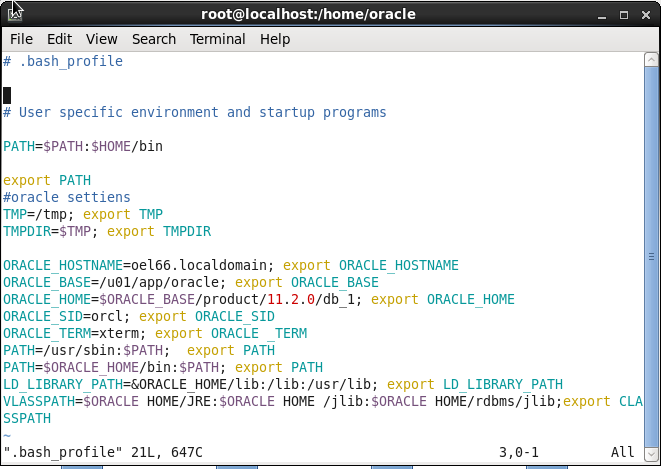
\includegraphics[width=14cm]{./Imagenes/img44} 
	\end{center}
	
	\item Ahora descomprimimos el archivo VT7489-01lof2.zip y el archivo VT7489-01lof2.zip . el cual creara una carpeta database como se muestra en la imagen
	\begin{center}
	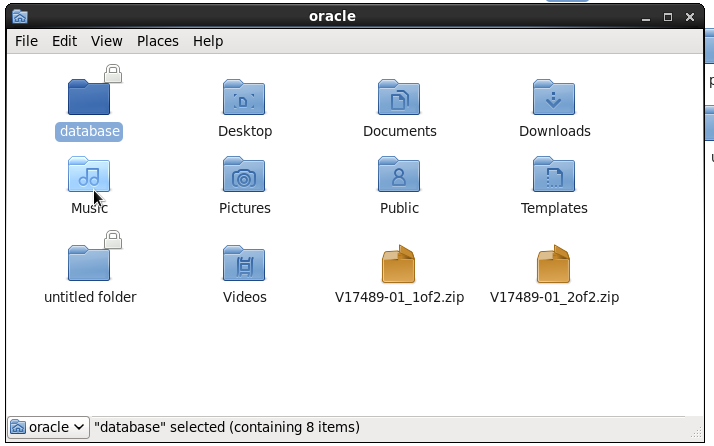
\includegraphics[width=14cm]{./Imagenes/img45} 
	\end{center}
\newpage
	\item Ahora iniciamos la instlacion de la base de datos Oracle haciendo doble clic sobre el archivo bash de instalacion y nos mostrara la siguiente venta presionamos en run, y saldra el menu de instalacion de de oracle.
	\begin{center}
	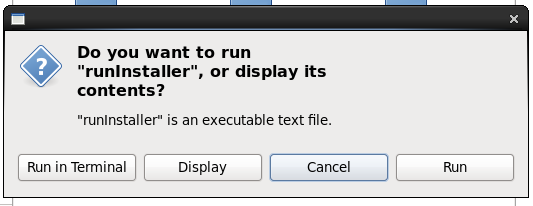
\includegraphics[width=14cm]{./Imagenes/img47} 
	\end{center}
	
	\item El menu de instalacion de oracle se mostrara como enla imagen en el cual escribiremos cualquier correo desmarcaremos el chek y presionaremos en siguiente para continuar la instalacion de la base de datos oracle.
	\begin{center}
	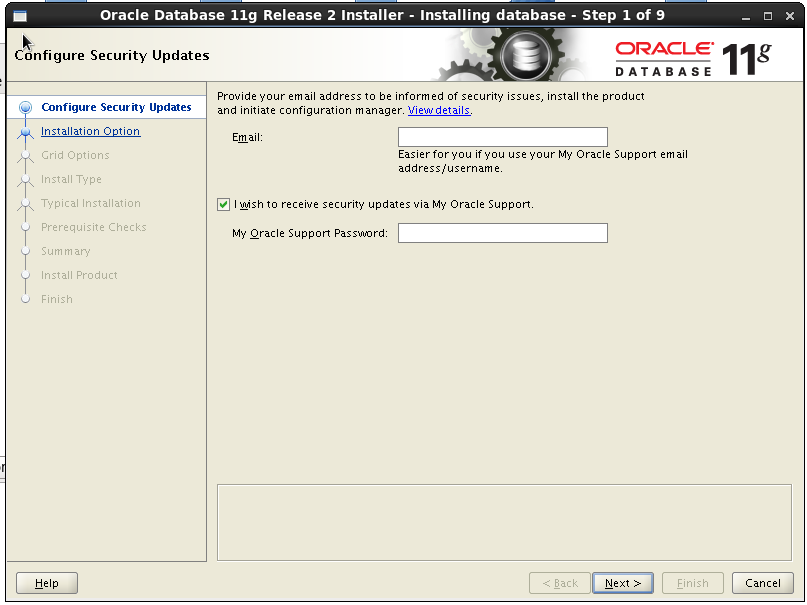
\includegraphics[width=14cm]{./Imagenes/img48} 
	\end{center}
\newpage

	\item Nos mostrara los siguientes de datos de instalcion elcual marcaremos el radiobutton de la opcion de crear y configurar una base de datos y presionaremos en siguiente.
	\begin{center}
	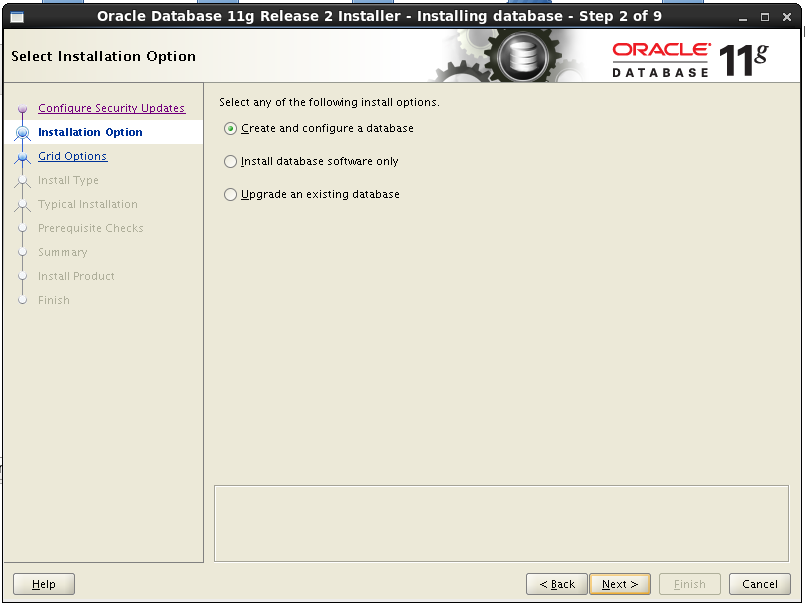
\includegraphics[width=13cm]{./Imagenes/img49} 
	\end{center}
	
	\item En este paso marcamos la opcion de server Class y preisonamos el boton de siguiente.
	\begin{center}
	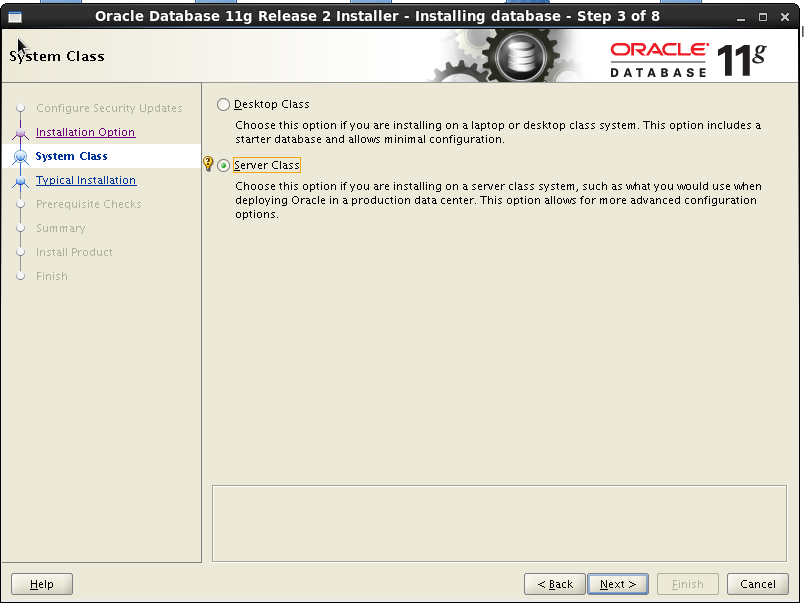
\includegraphics[width=13cm]{./Imagenes/img50} 
	\end{center}
	
\newpage

	\item Dejamos marcado la opcion por defecto y presionamos en el boton de siguiente para continuar con la instalacion de la base de datos oracle .
	\begin{center}
	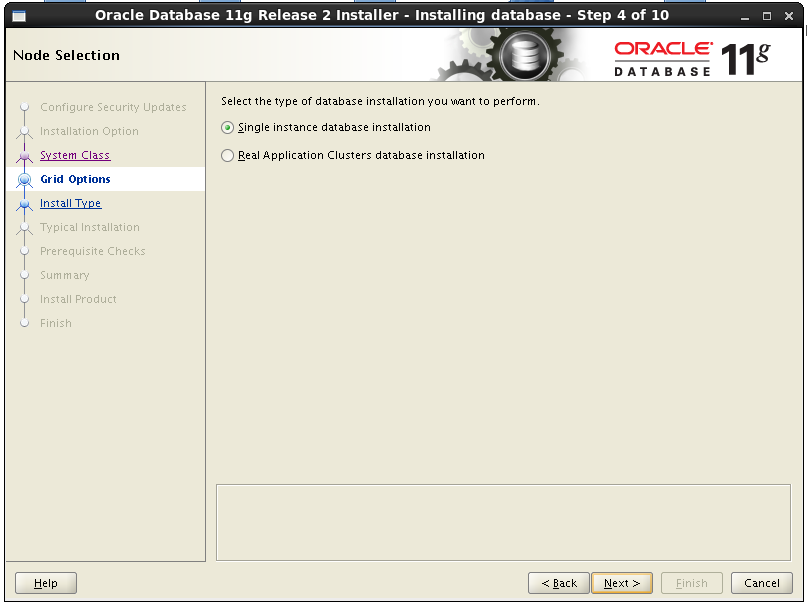
\includegraphics[width=13cm]{./Imagenes/img51} 
	\end{center}
	
	\item En este paso dejamos marcado la opcion de instalcion tipica y luego preisonamos la opcion de continuar.
	\begin{center}
	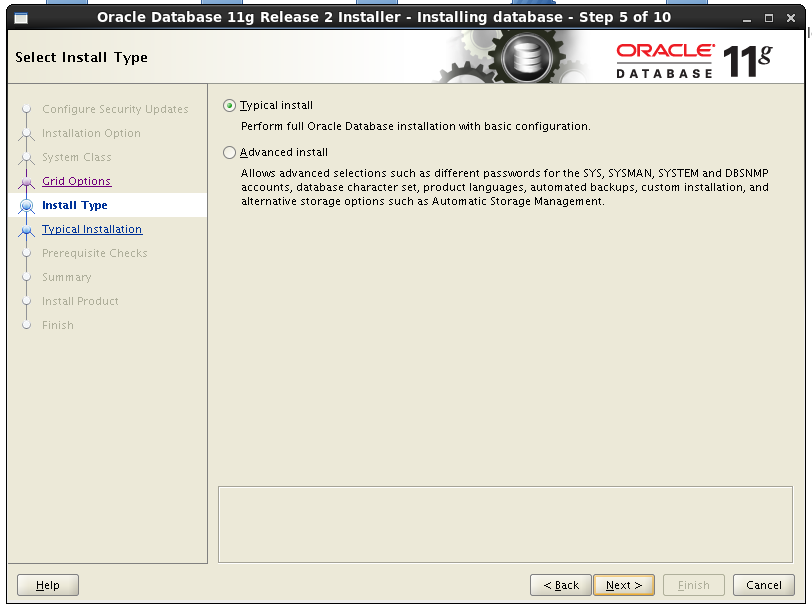
\includegraphics[width=13cm]{./Imagenes/img52} 
	\end{center}
	
	
\newpage

	\item Nos aparece la siguiente ventana el cual vamos a omitir este marcando la opcion de ignorar todo que se encuentra en la esquina superior derecha y el boton de siguiente se activara.
	\begin{center}
	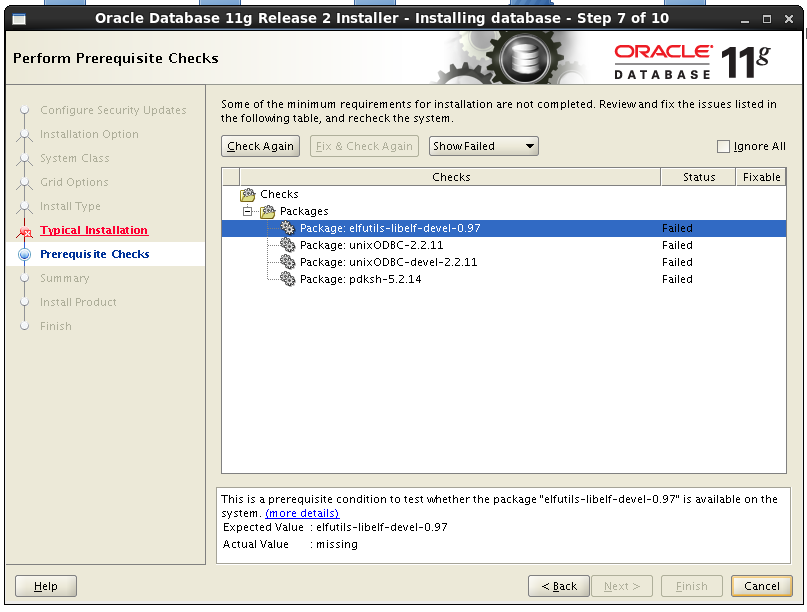
\includegraphics[width=13cm]{./Imagenes/img53} 
	\end{center}
	
	\item Nos mostrara un resumen de todas las opciones que emos selccionado .
	\begin{center}
	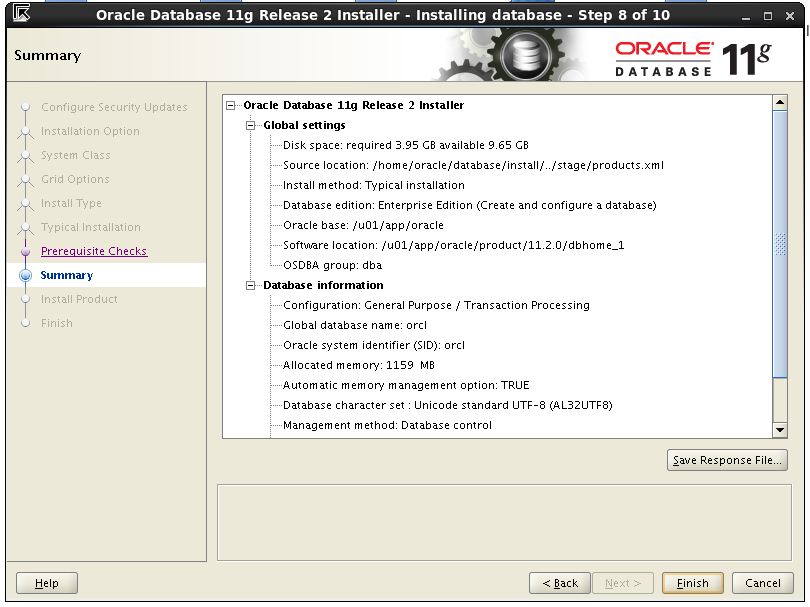
\includegraphics[width=13cm]{./Imagenes/img54} 
	\end{center}
	
	
\newpage

	\item Esperamos que la instalacion termine ,nos mostrara un cuadro donde nos muestra el estado de instalacion.
	\begin{center}
	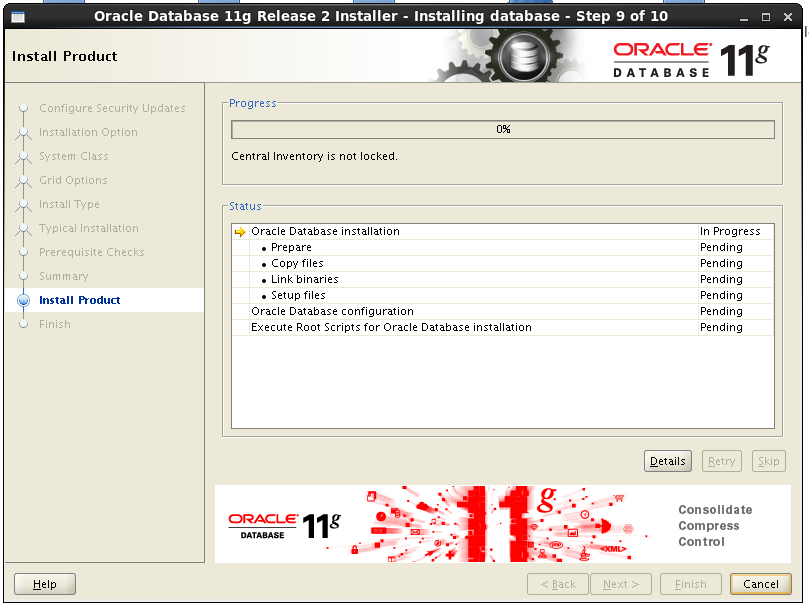
\includegraphics[width=13cm]{./Imagenes/img55} 
	\end{center}
	
	\item En este paso vamos a llenar los datos necesarios que nos pidepara continuar con la instalacion .
	\begin{center}
	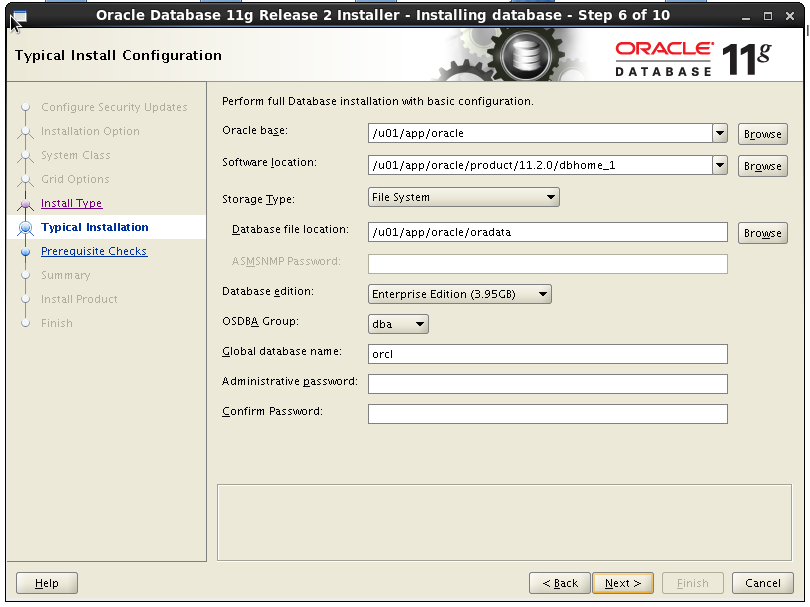
\includegraphics[width=13cm]{./Imagenes/img56} 
	\end{center}
	
	
\newpage

	\item Cuando estemos instalando la base de datos nos mostrara un mensaje que nos dice que se esta copiando la base de datos.
	\begin{center}
	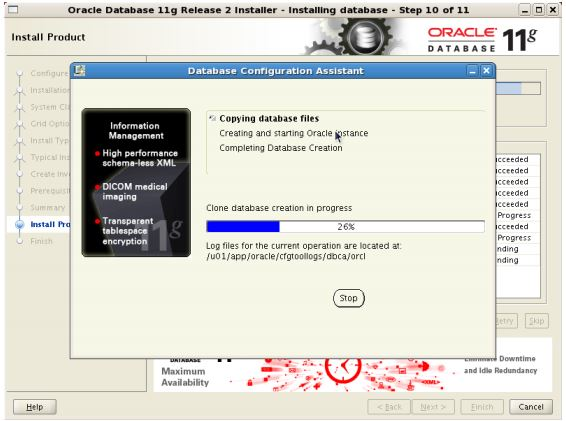
\includegraphics[width=13cm]{./Imagenes/img57} 
	\end{center}
	
	\item Al terminar la instalcion nos mostrara este mensaje donde nos muestra la informacionde la instalacion .
	\begin{center}
	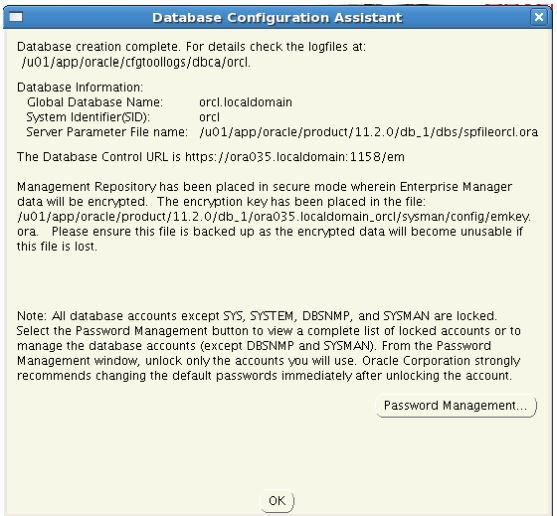
\includegraphics[width=10cm]{./Imagenes/img58} 
	\end{center}
	
	
\newpage

	\item Nos mostrara una ventana ,ahora cambiamos de usuario a usuario root y copiamos las dos rutas mostras a continuacion y pegaos en una terminal al final presionamos exit.
	\begin{center}
	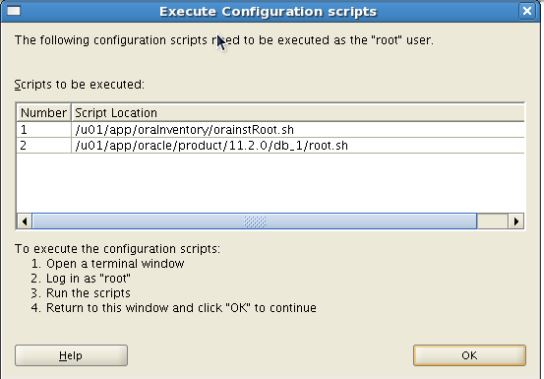
\includegraphics[width=13cm]{./Imagenes/img59} 
	\end{center}
	
	\item Nos saldra el mensaje de fin de la instalacion presionamos en exit   .
	\begin{center}
	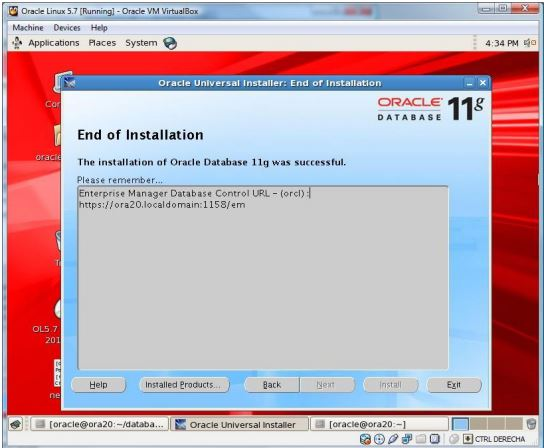
\includegraphics[width=10cm]{./Imagenes/img60} 
	\end{center}
	
\newpage

	\item Ahora tendremos que abrir un navegador y poner la siguiente direccion para que nos redireccione al gestor de base de datos de oracle.
	\begin{center}
	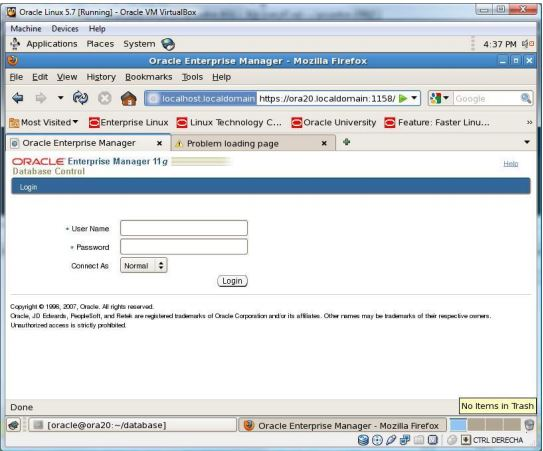
\includegraphics[width=13cm]{./Imagenes/img61} 
	\end{center}



\end{itemize} 
\newpage

\section{Cuestionario} 
	\item Los valores introducidos al archivo sysctl.conf ¿que representan?\\.
	fs.suiddumpable\\
    fs.aio-max-nr\\
    fs.file-max\\
    kernel.shmmni\\
    kernel.sem\\
    net.ipv4.iplocalortrange\\
    net.core.rmemdefault\\
    net.core.rmemmax\\
    net.core.wmemdefault\\
    net.core.wmemmax\\
   \item ¿Con qué usuario(s) puedo conectarme al servidor a través del AdministradorEmpresarial?\\
   Con el usuario SYS
